% A schematic example for the presentation template, not research evidence.
\documentclass[tikz,border=3pt]{standalone}
\usepackage{pgfplots}
\pgfplotsset{compat=1.18}
\begin{document}
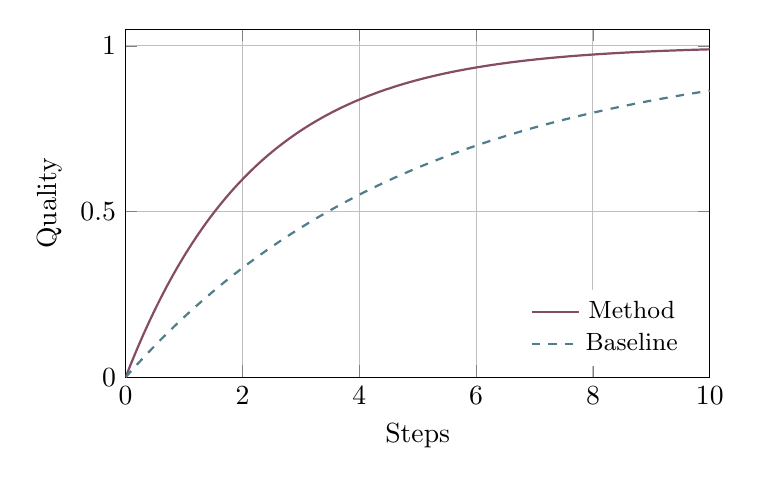
\begin{tikzpicture}
\begin{axis}[width=9cm,height=6cm,xlabel={Steps},ylabel={Quality},
 xmin=0,xmax=10,ymin=0,ymax=1.05,grid=major,
 legend pos=south east,legend style={draw=none,font=\small}]
\addplot[color={rgb,255:red,133;green,76;blue,101},thick,domain=0:10,samples=100]{1-exp(-x/2.2)};
\addlegendentry{Method}
\addplot[color={rgb,255:red,78;green,126;blue,140},thick,dashed,domain=0:10,samples=100]{1-exp(-x/5)};
\addlegendentry{Baseline}
\end{axis}
\end{tikzpicture}
\end{document}
